\documentclass[12pt,a4paper,draft]{article}
\usepackage[latin1]{inputenc}
\usepackage[english]{babel}
\usepackage{amsmath}
\usepackage{amsfonts}
\usepackage{amssymb}
\usepackage{graphicx}
\usepackage{appendix}
\author{Giuseppe Andronico}
\title{NN like method for JUNO positron events}
\begin{document}
\section{Description}
 The JUNO detector is assimilable to a sphere of radius $r_CD \approx 20 m$, see Fig. \ref{fig:eventdisplay}. The main goal of the detector is to study anti neutrino decays:
 \begin{figure}
 \centering
 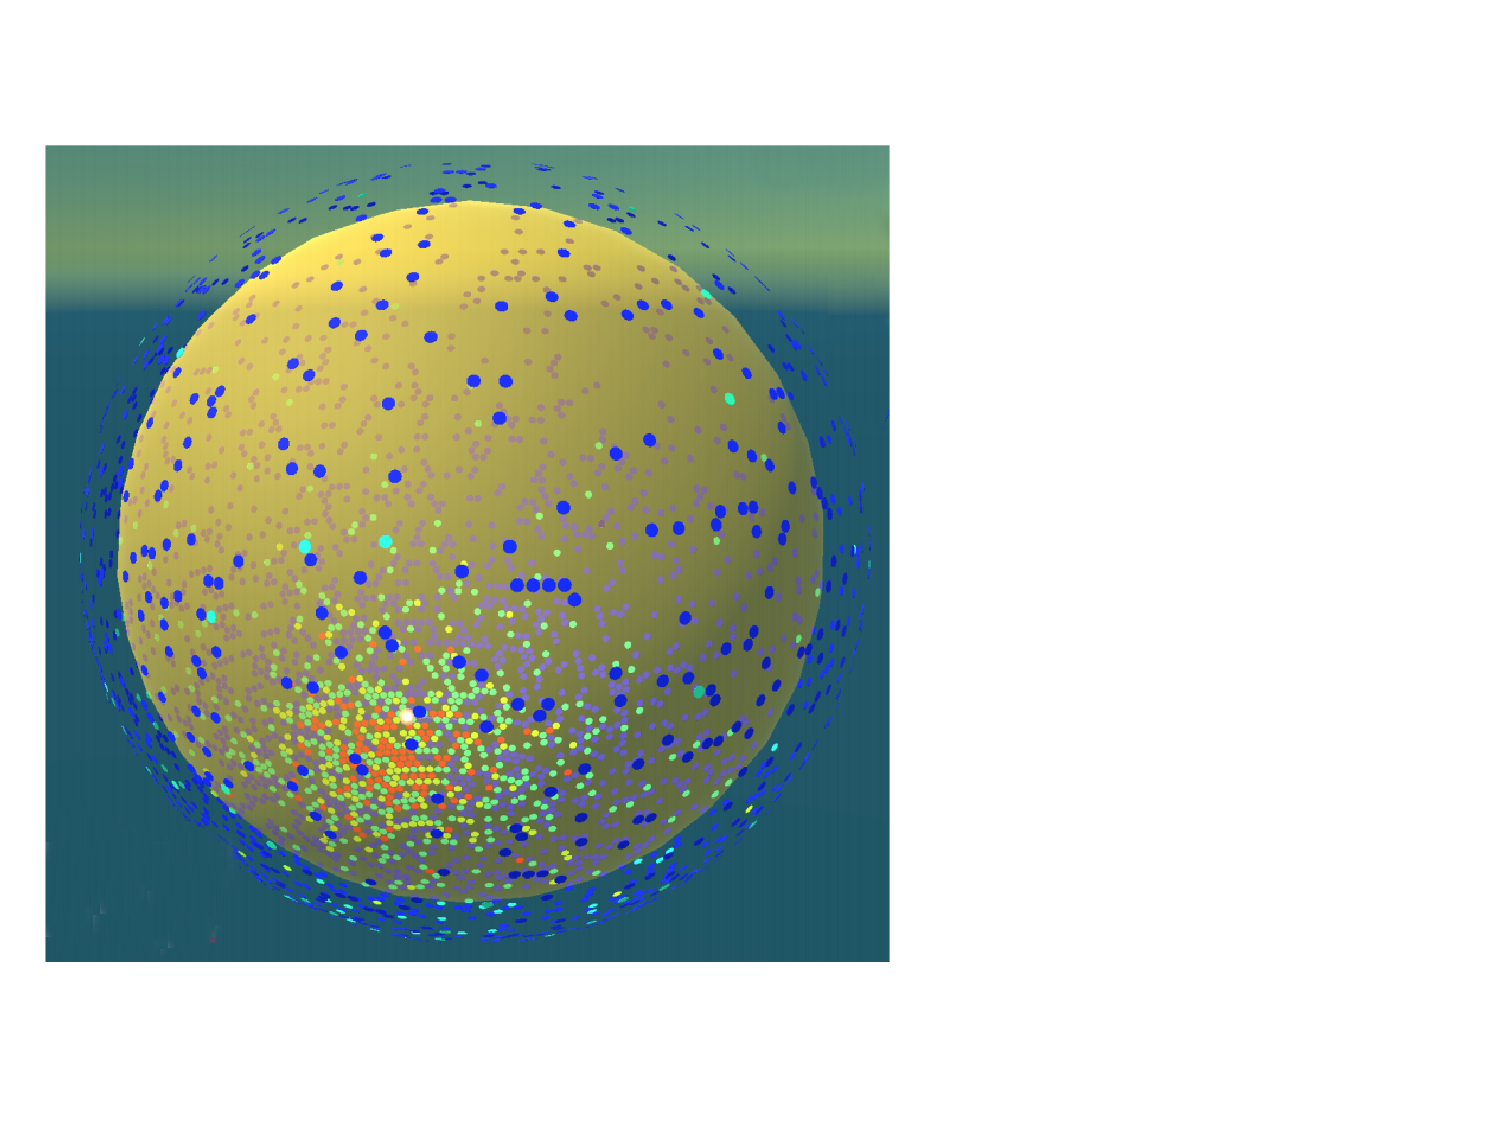
\includegraphics[]{images/EventDisplay}
% 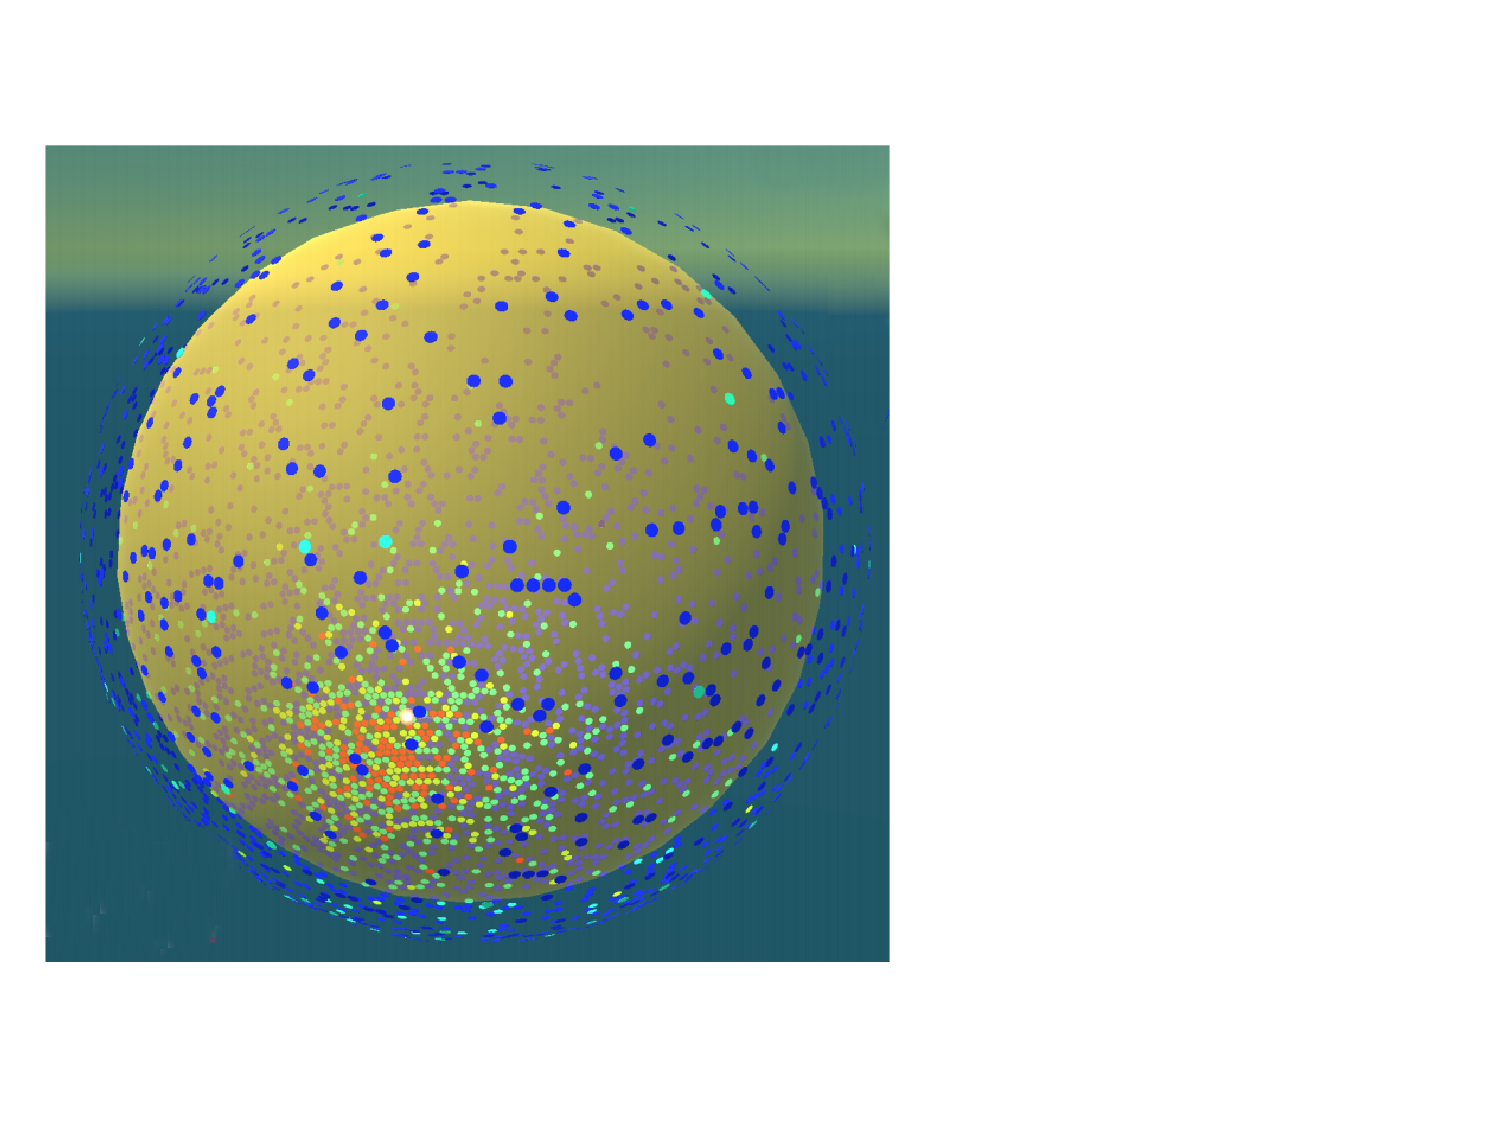
\includegraphics[width=0.7]{images/EventDisplay.png}
 \caption[Event in EventDisplay]{JUNO detector with fired PMTs in an event as view from EventDisplay}
 \label{fig:eventdisplay}
 \end{figure}
 \begin{enumerate}
 \item anti neutrino interacting with a proton produce a positron and a neutron
 \item the positron interacts with an electron in a point $A_ee = (x_ee,y_ee,z_ee)$ and both of them annihilates producing 2 gammas that will excite the liquid scintillator
 \item the liquid scintillator will produce light in the form of a spheric wave propagating from the annihilation point towards the sphere and the photo multipliers (PMT) attached on the external sphere surface
 \item the PMT will react with a signal proportional to the number of photons arriving on the device and in different times.
 \end{enumerate}
\section{Data selection for input}
 \subsection{Note: original data}
  Made from Yury. Description on slides 18-20 presented at January 2019 meeting. Produced with a flat distribution in positron kinetic energy, uniformly distributed inside CD. The script to generate events is \texttt{tut detsim.py}. The original files are at IHEP cluster in the path  \texttt{/afs/ihep.ac.cn/users/y/yury/spmt\_dir/yury/} in the folder \texttt{1M\_flat\_eplus}. The file with 1 million event is around 550 GB.\par
  To reduce size datasets have been processed
 Input come from Monte Carlo simulation, data stored on root files containing:
 \begin{enumerate}
 \item charge at each PMT
 \item hit time at each PMT
 \item PMT position.
 \end{enumerate}
 An attempt is:
 \begin{enumerate}
 \item to locate the first PMT to provide a signal and define a solid angle around this
 \item define a fixed number of points around the central point inside the solid angle
 \item for each of this points extract a limited number (4 or 5) of features from waveforms
 \end{enumerate}
\section{Selecting data from PMTs}
We defined a strategy to extract data. The basic idea is to select a limited number of PMTS and look at the waveforms in output from this waveforms.\par
the first step is to chosen the initial point $P_0 \equiv \left( \theta_0 , \phi_0 \right)$: we choose the first PMT to detect light. In fact the light emitted from the scintillator is isotropic, so the first PMT to detect light should be also the nearest PMT at the positron vertex.
From this point we can consider 
\section{Data output}
 The information that are desired in output are:
 \begin{itemize}
 \item Energy
 \item position
 \item positron momentum ?
 \end{itemize}
\appendix
\section{Angles and triangles}
Given a sphere of radius $r$, with center in the origin, a generic point on the sphere is $P \equiv \left( x, y, z \right) \equiv \left( r, \vartheta, \varphi \right)$ where:
\begin{align}
    x & = r \cos\left( \vartheta \right) \sin \left( \varphi \right) \label{sphericx}\\
    y & = r \sin\left( \vartheta \right) \sin \left( \varphi \right) \label{sphericy}\\
    x & = r \cos \left( \varphi \right)  \label{sphericz}
\end{align}
$\vartheta \in \left[0,2\pi\right)$, $\varphi \in \left[0,\pi\right]$.

Given 2 points on the sphere $P_1$ and $P_2$, we want to know the angle between the two radii going from $O$ to $P_1$ and from $O$ to $P_2$.
It is an isosceles triangle with the two equal sides being two radii. Be $a$ the segment from $P_1$ to $P_2$. Using \ref{sphericx}, \ref{sphericy}, \ref{sphericz} in the distance between two points formula we get:
\begin{equation}
    a = r \sqrt{6 - 2 \left[ \cos \left( \vartheta_1 - \vartheta_2 \right) \sin \varphi_1 \sin \varphi_2 + \cos \varphi_1 \cos \varphi_2  \right]} \label{iso_base}
\end{equation}

In the isosceles triangle $OP_1P_2$ the angle $\hat{P_1OP_2} \equiv \alpha $ and the two basis angles $\hat{OP_1P_2} \equiv \hat{OP_2P_1} \equiv \beta$ are related by
\begin{align}
    \beta & = \frac{\pi}{2} - \frac{\alpha}{2} \label{iso_angles}\\
    \sin{\beta} & = \cos{\frac{\alpha}{2}} \label{iso_sin}.
\end{align}
Using the relation between sides and angles in a triangle, that in our case is
\begin{equation}
    \frac{a}{\sin{\alpha}} = \frac{r}{\sin{\beta}} \Rightarrow{} \sin{\frac{\alpha}{2}} = \frac{1}{2}\frac{a}{r} \label{iso_vangle}
\end{equation}
Combining \ref{iso_vangle} and \ref{iso_base}, we get
\begin{equation}
    \alpha = 2 \arcsin \frac{1}{2} \sqrt{6 - 2 \left[ \cos \left( \vartheta_1 - \vartheta_2 \right) \sin \varphi_1 \sin \varphi_2 + \cos \varphi_1 \cos \varphi_2  \right]}. \label{arc_on_the_sphere}
\end{equation}
At this point we can consider the following problem: given a point on the sphere $P_0 \equiv \left( \theta_0 , \phi_0 \right)$, we want to find the points $P_1 \equiv \left( \vartheta_1 , \varphi_1 \right)$ on the sphere that form a given arc $\psi$ with $P_0$. By using \ref{arc_on_the_sphere} we get:
\begin{equation*}
    \psi = 2 \arcsin \frac{1}{2} \sqrt{6 - 2 \left[ \cos \left( \theta_0 - \vartheta_1 \right) \sin \phi_0 \sin \varphi_1 + \cos \phi_0 \cos \varphi_1  \right]}
\end{equation*}
where $\psi,\theta_0,\phi_0$ are known and $\vartheta_1,\varphi_1$ are the unknown variables. With a bit of trigonometry and algebraic we got a relation bounding $\vartheta_1, \varphi_1$:
\begin{equation}
    \vartheta_1 = \theta_0 - \arccos \frac{6-4\left(\sin{\frac{1}{2}\psi}\right)^2 - \cos \phi_0 \cos \varphi_1}{\sin \phi_0 \sin \varphi_1}. \label{relation_theta_phi}
\end{equation}

\end{document}